\section{Literature Review} % 2-3 Pages

% Gestures (Pointing (Dietic & Manipulative) vs Semaphoric)
%   Since used by the systems mentioned in the intro, discuss these 3 types
%   Examples of these gestures (with regards to systems referenced in intro)
%   Why you'd use them

% Tracking?
%   Examples of systems that use the head to interact with the phone (how they currently track the head), so can discuss the issue in more depth?
%   

% This something to go under design?
% Machine Learning / Gaussian Process / Particle Filters?

\subsection{Head Gestures}
% Mention types of gestures here, e.g. spatial vs semantic. Will be reviewing both, as will be intending to utilise both styles.

Gestures can be classified into 5 classes\cite{karam2005taxonomy}:
\begin{description}
    \item[Dietic] These are gestures that involve pointing, and mapping this to either a specific object or location within the interface.
    \item[Manipulative] A gesture which indicates intent to manipulate some object.
    \item[Semaphoric] Gestures which map to a specific action or intent.
    \item[Gesticulative] Typically accompany speech, but not required to transfer meaning.
    \item[Language] A substitute to written or verbal language.
\end{description}
For the purposes of this project, we shall be intending to review Dietic, Manipulative, and Semaphoric gestures to support user interaction.
\\\\
% Review of head gestures / study?
% Gestures as form of control
One of the simpler ways to track the movement of a user's head is with an Inertial Measurement Unit
 (IMU), as this is a physical device that can be used to measure rotational and linear acceleration\footnote{Linear acceleration is typically less accurately tracked compared to angular acceleration}.

An example of this can be seen in the work of \citeauthor{yan2018headgesture} who propose 9 gestures (\autoref{fig:yan2018headgesture_proposed_gestures}) and utilise the IMU embedded within the Hololens\cite{yan2018headgesture}.
\begin{figure}
    \centering
    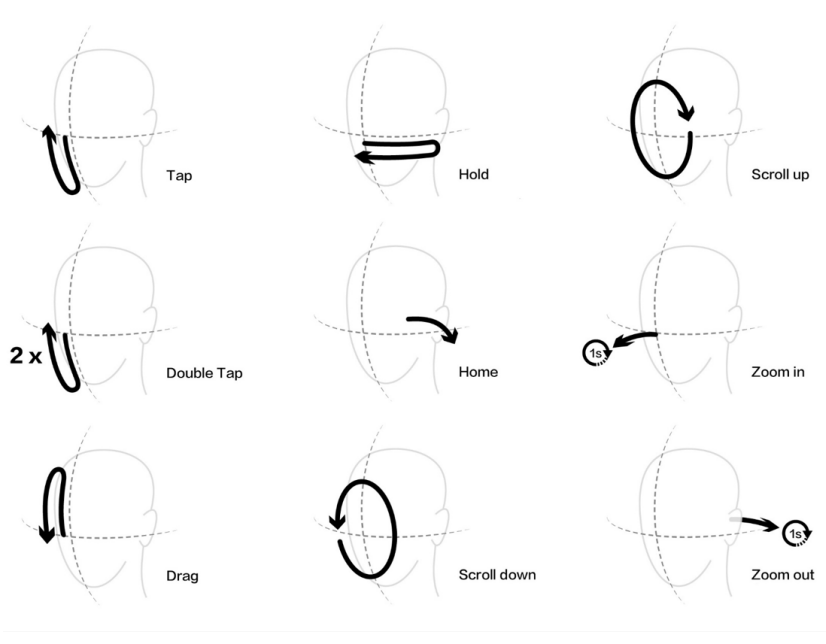
\includegraphics[width=0.5\textwidth]{figures/yan2018headgesture_fig2_proposed_gestures.png}
    \caption{\label{fig:yan2018headgesture_proposed_gestures} Proposed head gestures and their corresponding actions\cite{yan2018headgesture}.}
\end{figure}

The gestures they propose were derived from a study wherein they asked participants to suggest head movements that they believed corresponded to the action taken.
These were then collated by manually into 80 gestures, which were then effectively voted upon by the participants for their respective actions.
The gestures with the most votes for a given action were selected, with some minor adjustments to ensure there were no clashes between actions.

To extract the gestures from the Hololens, the IMU output was segmented via detection of acceleration (20 degrees per second) and deceleration (4 degrees per second), not exceeding 2 seconds.

Feature extraction is performed with Dynamic Time Warping (DTW)\cite{berndt1994using}, followed by a Support Vector Machine (SVM) classifier to classify the observed gesture into one of 9 the categories, or unintentional movement. With just the DTW they were able to achieve 90\% accuracy, but with the SVM they were able to boost this to 97\%.

To evaluate the head gestures, they compared them with existing hand gestures. They found that head gestures caused more fatigue and generally felt less natural, while being equivalent or better with regards to learnability.

% Gestures as interface interactions
% Closer to mobile, as have just reliance on cameras
Using a mobile device we won't have access to an IMU on the user's head, however we will be able to try and utilise the same set of gestures, and to use a similar approach to track the phone's movement, which could allow us to try and differentiate between the phone or head being moved.
\\\\
An alternative approach is to try and extract the face using an RGB camera.

One way to do this was developed by \citeauthor{gorodnichy2002importance}, which 'finds' the nose under the assumption that it should have the greatest intensity gradient since it should always be closest to the camera, and given it is convex in nature it should be the 'brightest' feature\cite{gorodnichy2002importance}.

The tracked point isn't a specific point on the nose (e.g. the tip), but a point that can move across the surface of the nose, based on what is closest to the camera.

They go on to extend this work with the usage of the user's nose to control a pointer on their screen\cite{gorodnichy2004nouse}. 
They extract just the nose since it meets their two requirements for a trackable feature: \begin{enumerate}
    \item It is always visible, presuming the user is facing within 180 degrees towards the camera.
    \item Only one feature should be used to define the cursor, to reduce/eliminate potential jitter.
\end{enumerate}

To click with the 'Nouse' the user blinks twice within short succession. Blinking is determined by reviewing the change in the sequence of 3 frames.

To ensure the system is realtime they use a reduced resolution, and could find that a resolution of 160x120 was robust enough to accurately track nose, and map the cursor to an accurate location on the screen.

They make claims about accuracy and enjoyment, but relevant data not provided. They only seemed to make statements suggesting Nouse was as good as, if not better than, typical mouse control.
They claim mouse usage caused wrist ache, but movement of entire head doesn't present neck ache, which was reported in the IMU head tracking describe4d above\cite{yan2018headgesture}.

Another nose controlled cursor is presented by \citeauthor{varona2008hands}, however they use Haar cascades to extract the region containing the face, within which they use a similar technique as above\cite{gorodnichy2002importance} to extract points for the corners of the nose, or the nostrils\cite{varona2008hands}.

To detect eyes, the system determines the user's skin colour by sampling the pixels within the detected face region. They then presume the eyes will be a different colour, and as such filter based on the extracted skin-tone. They then select the features closest to the nose, that are symmetrical.

A UI is provided with possible actions as buttons. The user moves the cursor to the action they wish to perform, then wink (with either eye) to select it. When they then fixate on part of the screen (move the cursor to a point and keep it stationary), the action will be performed.

Only evaluated for click recognition and accuracy of where the click was performed within a grid of points. However >80\% accuracy even for users with no training time, just instructions.

Moving closer to a tool for mobile devices we have the work of \citeauthor{roig2015face}, who use the front faced camera to scroll, using the head angle w/r/t the device as direction of scrolling.\cite{roig2015face}

They extend upon the work of \citeauthor{varona2008hands}\cite{varona2008hands} the nose of the user and to correlate it's motion to a virtual cursor on the screen.

Selection/tapping is performed via tapping anywhere on the screen, however the tap will actually occur under the virtual cursor.

They evaluated the system by asking users to select elements of varying sizes, phone held in different orientations (portrait vs landscape), and with varying gain applied to the velocity of the cursor in response to head movement.

Elements below 88x88pt\footnote{Apple Point, effectively 2 pixels on a retina display, so 88pt == 176px} were found to be less successfully selected, this is primarily due to the low resolution used for the gesture tracking being unable to be mapped to a finer resolution on the device screen. Potentially increasing the resolution used for the tracking could permit finer accuracy.

They do not distinguish between the user moving the phone, or the user moving their head. It could be seen as a feature, either move the phone or head to scroll, but this would be intersting to try and distinguish, to potentially support additional actions/gestures.

The above systems describe the ability to identify where on a screen the user is looking, or at the very least intends to perform some action, through providing them with a virtual cursor they can manipulate via moving there head, either through rotation or physically moving the head.
We can look to extend upon this to understand where the user's attention may be focused.
\\\\
Some smartphones now also include front-facing depth cameras, a technique for tracking a user's head, and detecting head/facial features is provided by \citeauthor{deepateep2020facial}, wherein they utilised the ARKit Framework for iOS\cite{deepateep2020facial}.

Objective similar to works described above to control a virtual cursor, however instead of specifically using the nose, they are using the perceived pose of the user's entire head.

Cursor motion is tracked based on head pitch and yaw in the Y and X directions respectively. Requires user to directly face the camera for zero movement of the cursor.

Additionally they combine this control with facial gestures, which perform specific actions, or permit the beginning of specific actions, such as zoom, drag, and tapping.
These utilised poses obtained from the eyebrows and mouth. Timings specific to each action, some gestures overloaded based on timing.


A depth camera affords greater accuracy for tracking (particularly for understanding the distance from the screen), and in case of iPhone there is consistency with specific hardware. 
However for the general smartphone population, specifically android, depth cameras aren't standard, and when present can have different hardware. 
For our project we will presume 3D depth cameras aren't available.
% Spatial 
% \cite{voelker2020headreach} developed a tool to combine head orientation to move a cursor into a particular section of the screen, from which they can then use relative motion of the thumb to adjust the cursor to the element of interest.\\
% Utilise the ARKit Framework for iOS.\\
% Utilise 3D-Touch (on Apple device used, application of force can be used to differentiate between a light or heavy touch) to activate the head-tracking mode.
% They presume that when mode engaged that user is facing phone to the extent they wish, and use this to calibrate the 'origin' position of the user's head, rather than requiring the user to face the camera.\\
% Tested 3 different interaction techniques.
% Head Cursor Only - once mode engaged, user moves head to where they want to select, and upon release current target is selected.
% Head Cursor and Touch - move cursor in same way, but applying more force then allows them to move their thumb to make adjustment to the cursor position.
% Head Area and Touch - rather than having a cursor controlled by the head, the head is used to select a quadrant of the display, then as with above technique the user can then move the cursor with their thumb to select a specific target.\\
% They compared this with direct touch and an existing thumb-only technique called BezelCursor \cite{li2016bezelcursor}, which permits a user to move a virtual cursor along the entire screen with just movements of their thumb.\\
% They found that while standing, direct touch was fastest, followed by the head tracking methods, with the BezelCursor being slowest. However accuracy was effectively reversed in order.\\
% While walking this was similar, however the Head Cursor Only approach was slowest overall and less accurate than direct touch.

% % Semantic & Spatial
% This was then extended upon \citep{hueber2020headbang} to use the same tracking technology to instead perform gestures.\\
% activated by lightly touching the element, followed by performing the gesture. The detected action is shown as a pop-up and can be selected by releasing the touch, or cancelled by moving the touch out of the element and then releasing.\\
% Gestures were made simple based on the direction the user looked away, with actions effectively being placed within a disk, with each action getting an equally sized segment.
% Performing a gesture requires a user to remember the direction associated with the action they wish to perform.\\
% Then then compared to other techniques that work off similar principle (using a segmented wheel to represent different actions), some requiring the device itself be moved, or the thumb, and one other technique that instead uses a vertical list in-place of a wheel.\\
% HeadBang was observed with the greatest accuracy of the wheel segmented approaches for all menu sizes, however was out-performed by the vertical list for all but the smallest menu size.

% Fair to say, or need data proof?

% Basically what we were thinking of doing, but without an adaptive interface...
% Spatial 
% \cite{hansen2006use} Tool to use front-facing camera to track phone movement relative to user's face.
% Face extracted through histogram (user places face in centre of frame and clicks button to calibrate their skin-tone), it then determines the range of hue for the face based on a region of pixels in the centre of the frame, and uses this to bin the pixels into face and background based on the hue.\\
% The size, centre and rotation of the extracted region is then computed, this is remembered between frames to reduce the impact of changes in background, as 
% They then use this input to evaluate 3 applications (image viewer, Bluetooth connections, pong).\\
% They highlight that there is an issue with moving device vs tilting, but offer no solution, camera FOV can reduce action-space, and that accessibility issues with moving the phone, making it harder to read.

% \subsubsection{Types of Gestures} % Before or after Mobile devices?

% \cite{aigner2012understanding} Types of gesture

% From the head gesture systems reviewed above, we can classify them into 2 groups of gesture types.
% Summarising from \pcite{clarke2020dynamic} thesis, gestures can be defined as being "semantically mapped to a set of corresponding actions", or Spatially mapped, although the gestures themselves may occur spatially in motor space. Manipulative and pointing gestures involve a spatial mapping, and usually a logical abstraction of the user’s attention in the form of a cursor"
% \begin{description}
%     \item[Semantic] Wherein the gesture is mapped to a specific action within the action space. Such as a static hand-pose (e.g. thumbs-up), or a specific sequence of poses (e.g. 
%     \item[Spatial]  The gesture is mapped to some value-space, the value corresponds directly to the gesture pose. Such as the movement of a pointer on a screen, or the position of a slider or dial.
% \end{description}


\subsection{Adaptive Interfaces}
% Start with general examples, then refine towards mobile devices, then if possible, refine to head controlled

% \cite{wesson2010can} Describes the types of adaptive UI (e.g. what contexts the UI is aware of) 

\subsubsection{3D Interfaces} % Projected to 2D display
% An alternative to tabs/pages in applications, have application interface in 3D, and only expose based on perspective
% Perspective based on phone vs user
% Examples of AR/VR, display adapts

% \cite{buschel2017investigating} Using IR camera array and trackable tablet (attachments to track via IR cameras), track the 3d position and rotation of device within space.\\
% Position and rotation then used to adjust the rendered view of the 3D graphs (though could be extended to more 3D models generally). Allows user to view different perspectives and focus on specific regions though physical movement of the device, rather than with just touch input.\\
% Compared 3 different tasks (finding specific information, comparing size of objects, and structural understanding (selecting a similar plot))\\
% Fatigue was highest for the device movement, compared to touch, however outperformed touch significantly with regards to perceived control of the viewport, and perceived success.\\
% They couldn't find any significant difference in completion times or success rate for the comparative and structural understanding tasks, but could observe that the navigation task was generally completed faster when utilising the touch only interface. this could be due to the size of the virtual environment, requiring users to move to find items, while touch interaction permitted zooming out and then back in.
A 3D interface presumes that there is a virtual screen through which a portion is visible from the mobile device.

\citeauthor{francone2011using} approaches this by developing a system which adjusts 3D content on the screen based on the user's perspective/orientation relative to the phone screen/front facing camera\cite{francone2011using}.

Their system utilises Haar cascades to extract the user's face. The X and Y positions are tracked via the centre of the observed bounding box. Here they intentionally accept both movement of  either the head or device.
Depth is estimated via the size of the region, however this fails if the user's face starts to go out-of-frame of the camera, as the a portion of the face may still be recognise, resulting in a thin bounding box.

For their interface they tested:
\begin{itemize}
    \item Displaying 3D interface elements, e.g. adding depth to the interface such that adjusting perspective would permit viewing the sides of elements within the UI.
    \item A workspace that was too large to fit onto the screen, and to reveal other elements of the interface you could adjust the perspective, rather than say changing the page.
\end{itemize}
For their evaluation they did not compare with existing techniques, such as touch, but rather asked participants to directly evaluate the usability in isolation.

We can learn from \citeauthor{francone2011using} regarding the depth axis. To alleviate the issue wherein the face is partially out-of-frame we could adjust the face detection to require the whole face, or to understand how much of a face has been detected.
We can also follow a similar evaluation procedure, however it would be beneficial to also compare to an existing interface.
\\\\
Another approach is developed by \citeauthor{miyazaki2021ar}, however they approach this from the perspective of the phone moving to expose a virtual display\cite{miyazaki2021ar}.

They developed a virtual display (a map within which several 'pins' are present), which could either be viewed as static and hovering in-front of the user, or placed upon a 2D plane in their environment.
To move around the virtual display, they simply need to move the device.
To do this they utilised Google's Ar toolkit: Tango. The rear camera of the device would be used by Tango to track the device, and to track the position of the virtual display, either with respect to a 2D plane, or the user.

They evaluated these two displays against a touch-only display, which could only be manipulated by touch.
They found that the touch only implementation was the slowest for finding various the pins.
Both virtual display interfaces were found to require less mental load (like recalling the direction of various points on the map from the current position), and intuitive to use when compared with touch only, though the non-AR instance was found to be more taxing to use.

For our project we can look into also utilising some AR features to help track the phone, and differentiate the movement of the head vs movement of the phone.
However we would need to investigate power usage and processing limits if we are trying to perform AR tracking and head tracking, using both front and rear cameras.

\subsubsection{Context Aware UI}
% One way to improve usability is to have the UI elements adapt to the user context
% based on:
%   prior actions
%   current area of focus (enlarging / moving elements to make easier for user to interact)
%   user goals

% AR
Where the 3D UI allows a user to move around and adjust the perspective of the UI elements, an alternative approach would be to instead change which UI elements are on screen in reaction to the user's attention or perceived intentions.

An example of this by \citeauthor{pfeuffer2021artention} is a UI for an AR head mounted display which adjusts the displed content and presented information based on user's gaze\cite{pfeuffer2021artention}.

This is primarily controlled via user gaze, specifically dwell-time, however is also informed by the task context.
For example in their conversational UI, information about a person is presented around them, in the background, however if the user were to dwell upon specific information, it will bring it to the foreground, and display more (if applicable), until they revert their gaze back upon the person.
In the tree of life example (a network graph for a subset of the tree of life is rendered), there is no 'background', instead gaze is used to adjust the level of information for specific nodes.
This is also the case for the shopping interface, where gaze permits information to display for specific items, and the ability to interact with said items.

They evaluated their interfaces with different amounts dwell-timerequired to adapt/accept user input, to compare the accuracy and error rate.
With shorter dwell times task completion was faster, as expected, but the error rate much higher. They found that a 3 sec dwell-time was least error prone (in a range of 1-4s).
However the majority of participants found the dwell-time was too slow for anything beyond 2s.

We can't use this directly, as we won't be using gaze, but we could adapt to work with a cursor controlled by the user's head.
\\\\
% Gestures more generally ?
% \cite{clarke2020reactive} adapts presented video based on gesture recognition

% Specific to mobile device
% The work by \citeauthor{yigitbas2019context} \cite{{yigitbas2019context, yigitbas2019component}} evaluate 2 similar applications that react to various user environment states, and previously learned information about the user.
% Second one can be dropped?
% Specific to head reaction
Another interpretation of this is the interface developed by \citeauthor{lopez2012head}, which is a virtual display that is in the shape of a concave box, from which the visible part of the box is based on the user's perspective.\cite{lopez2012head}. 
This is similar to the work of \citeauthor{francone2011using}, however specifically for extending workspaces, and for supporting adaptive UI elements which react to the user's head position.

One interface is described as being a concave box, from which interface elements are placed. When the user places attention to a particular element, it is brought into the foreground for use, and can then be dismissed for them to select another element.
Another interface they describe permits head gestures to be recognised which map to revealing additional UI elements based on user intent. Their example involves a web-page, wherein turning/moving in from the right would reveal a prompt to add the page to the bookmarks, and continuing the motion would open the bookmark dialogue.
% Also looks into whether the head or phone moving

The head is extracted via an Adaboost classifier which determines the weighting of a 20x20px neighbourhood of pixels as containing facial features, in similar manner to Haar cascade.
head distance is then estimated via change in scale of the extracted region, so no definitive size, but permits a relative scale/distance from original size.

Due to limited Field of View (FOV) of the camera, they added a wide-angle lens to increase the FOV to 160 degrees.

Unfortunately they don't actually implement an instance of any of their proposed interfaces, which is something we can look to achieve and evaluate.


% Summary?

%% QUOTES & NOTES %%


% Two points of interest:\\
% - Input modalities: to address limited reach of thumb\\
% - Adaptive Interfaces: To adjust visible elements / positioning of elements based on context\\

% % Would start with thumb gestures, but is this needed?
% % Can look to combine head movement with thumb?
% % Start with more cumbersome / excessive gestural techniques, refine towards thumb + head/gaze

% % Discuss determining if head vs phone is moving

% \subsection{Input Modalities}
% \subsubsection{Phone Gestures}
% % @inproceedings{ti2013tiltzoom,
% %   title={TiltZoom: tilt-based zooming control for easy one-handed mobile interactions},
% %   author={Ti, Jimmy and Tjondronegoro, Dian},
% %   booktitle={Australian Computer-Human Interaction Conference (24th)},
% %   pages={1--1},
% %   year={2013}
% % }
% Though limited in functionality, \pcite{ti2013tiltzoom} TiltZoom tool permits a user to adjust the level of zoom of a map via tilting the phone away (zoom-out) and towards (zoom-in) the user.\\
% This is due to typical zooming gestures requiring 2 digit input (e.g. pinching the display), which often requires two-handed interaction with the phone.

% Though apps such as google images and maps now support a double-tap and drag gesture to perform zoom operations, the usage of physical device rotation did show that it could be a usable and accessible user input.\\
% However one downside that was observed was a tiring of the wrist.

% % @inproceedings{chen2012extending,
% %   title={Extending a mobile device's interaction space through body-centric interaction},
% %   author={Chen, Xiang'Anthony' and Marquardt, Nicolai and Tang, Anthony and Boring, Sebastian and Greenberg, Saul},
% %   booktitle={Proceedings of the 14th international conference on Human-computer interaction with mobile devices and services},
% %   pages={151--160},
% %   year={2012}
% % }
% \cite{chen2012extending} took a different approach to phone-based gestures. Rather than developing a technique to convert the phone positioning/movement into an analog input, they instead looked to develop a system that used fixed / incremental input, that treated the phone position relative to the body as an action\\
% More akin to pressing max / min volume vs slowly incrementing the volume.\\
% Their system permits users to 'place' objects (such as urls, images, calender appointments) with respect to their body, which can then be retrieved at a later time.\\
% This could be interpreted as having a virtual space around the body, wherein the phone acts as a cursor to interact with elements within the space.

% \subsubsection{Head Gestures}
% Either tracking head / face to act as a pointer, or to be interpreted as a gesture.
% % Spacial and semantic input

% % @inproceedings{roig2015face,
% %   title={Face Me! Head-tracker interface evaluation on mobile devices},
% %   author={Roig-Maim{\'o}, Maria Francesca and Varona G{\'o}mez, Javier and Manresa-Yee, Cristina},
% %   booktitle={Proceedings of the 33rd Annual ACM Conference Extended Abstracts on Human Factors in Computing Systems},
% %   pages={1573--1578},
% %   year={2015}
% % }
% \cite{roig2015face} Using front faced camera to scroll, using the head angle w/r/t the device as direction of scrolling.\\


% % @article{onuki2016combined,
% %   title={Combined use of rear touch gestures and facial feature detection to achieve single-handed navigation of mobile devices},
% %   author={Onuki, Yoshikazu and Kumazawa, Itsuo},
% %   journal={IEEE Transactions on Human-Machine Systems},
% %   volume={46},
% %   number={5},
% %   pages={684--693},
% %   year={2016},
% %   publisher={IEEE}
% % }
% \cite{onuki2016combined} Using front facing camera to track user's head orientation (used to move a cursor), and the distance between the user's eyes to infer distance from the display, which in turn adjusts the coarseness of the cursor locations by effectively zooming in/out.

% % @inproceedings{voelker2020headreach,
% %   title={HeadReach: Using Head Tracking to Increase Reachability on Mobile Touch Devices},
% %   author={Voelker, Simon and Hueber, Sebastian and Corsten, Christian and Remy, Christian},
% %   booktitle={Proceedings of the 2020 CHI Conference on Human Factors in Computing Systems},
% %   pages={1--12},
% %   year={2020}
% % }
% \cite{voelker2020headreach} developed a tool to combine head orientation to move a cursor into a particular section of the screen, from which they can then use relative motion of the thumb to adjust the cursor to the element of interest.\\

% % @inproceedings{hueber2020headbang,
% %   title={Headbang: Using head gestures to trigger discrete actions on mobile devices},
% %   author={Hueber, Sebastian and Cherek, Christian and Wacker, Philipp and Borchers, Jan and Voelker, Simon},
% %   booktitle={22nd International Conference on Human-Computer Interaction with Mobile Devices and Services},
% %   pages={1--10},
% %   year={2020}
% % }
% This was then extended upon \citep{hueber2020headbang} to use the same tracking technology to instead perform gestures.\\
% Gestures were made simple based on the direction the user looked away, with actions effectively being placed within a disk, with each action getting an equally sized segment.\\
% Performing a gesture requires a user to remember the direction associated with the action they wish to perform.
% % Unclear if tested success using different number of segments

% Unsure if any of the above could determine if head or phone was being moved/rotated

% % @article{yan2018headgesture,
% %   title={Headgesture: hands-free input approach leveraging head movements for hmd devices},
% %   author={Yan, Yukang and Yu, Chun and Yi, Xin and Shi, Yuanchun},
% %   journal={Proceedings of the ACM on Interactive, Mobile, Wearable and Ubiquitous Technologies},
% %   volume={2},
% %   number={4},
% %   pages={1--23},
% %   year={2018},
% %   publisher={ACM New York, NY, USA}
% % }
% \cite{yan2018headgesture} also developed a system for performing gestures with the user's head, however they utilised more complicated gestures. Made for hands-free, rather than extending touch input.\\
% They determined the gesture movements via a study, resulting in 9 gestures/actions.\\
% Each action was to be a substitute for an existing gesture that could be performed with touch, such as tapping, scrolling, and zooming.\\
% Tracking was performed with hololens (not from phone).\\
% Was evaluated against Air-Tap, hololens extracting hand gestures.


% % @inproceedings{hansen2006use,
% %   title={Use your head: exploring face tracking for mobile interaction},
% %   author={Hansen, Thomas Riisgaard and Eriksson, Eva and Lykke-Olesen, Andreas},
% %   booktitle={CHI'06 Extended Abstracts on Human Factors in Computing Systems},
% %   pages={845--850},
% %   year={2006}
% % }
% % Basically what we were thinking of doing, bu without an adaptive interface...
% \cite{hansen2006use} Tool to use front-facing camera to track phone movement relative to user's face.
% They then use this input to evaluate 3 applications (image viewer, bluetooth connections, pong).\\
% They highlight that there is an issue with moving device vs tilting, camera FOV can reduce action-space, and that accessibility issues with moving the phone, making it harder to read.

% \subsubsection{Gaze / Eye Tracking}

